\chapter{Tecnologie di interesse}
\label{cap:chapter3}

Questo capitolo si occupa di spiegare le tecnologie che sono state impiegate durante il tirocinio, al fine di comprendere successivamente le scelte progettuali intraprese durante lo sviluppo.
\\Particolare attenzione sarà dedicata agli standard definiti dall'Open Geospatial Consortium (OGC), tra cui Web Map Service (WMS), il Web Map Tiles Service (WMTS), Web Feature Service (WFS) e Web Coverage Service (WCS). Si tratta di protocolli universalmente riconosciuti per la distribuzione e l'accesso ai dati geospaziali tramite Internet.
Saranno inoltre analizzate altre tecnologie rilevanti per la gestione e la visualizzazione di dati geospaziali (come GeoJSON e ShapeFile), formati comuni per lo scambio di dati geografici.
% todo: rifare l'introduzione

\section{Gli standard forniti da OGC}

Il consorzio Open Geospatial Consortium (OGC) ha definito diversi standard per i servizi web che consentono ai client di accedere e interrogare informazioni geografiche. Tra questi troviamo:
\begin{itemize}
      \item Web Map Service (WMS);
      \item Web Map Tile Service (WMTS);
      \item Web Feature Service (WFS);
      \item Web Coverage Service (WCS).
\end{itemize}
Come spiegato nella documentazione \cite{DocumentazioneOGC}, ciascuno di questi standard offre funzionalità specifiche per soddisfare varie esigenze di accesso ai dati geospaziali. Questi servizi si basano su altre tecnologie come l'architettura REST e il protocollo SOAP, ai quali si accede dal client attraverso messaggi XML.

\begin{figure}
      \centering
      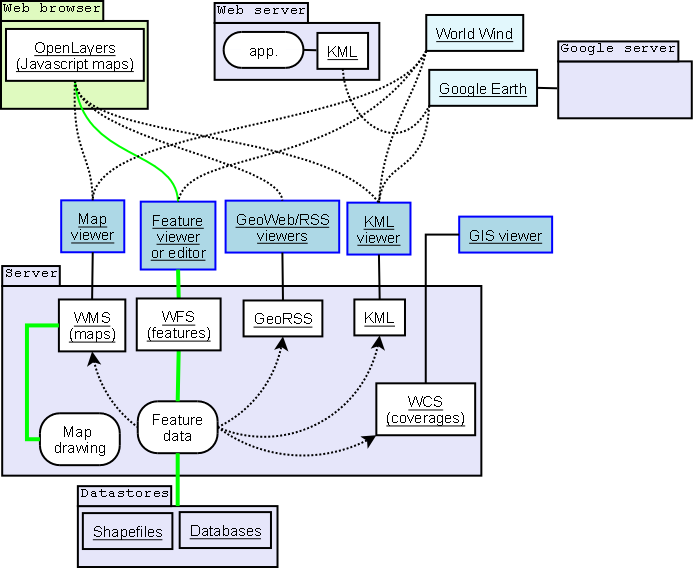
\includegraphics[width=0.8\textwidth]{images/Capitolo2/OGC.png}
      \caption{Relazione tra client/server e protocolli OGC}
      \label{fig:Relazione tra client/server e protocolli OGC}
\end{figure}
Lo standard OGC prevede che tutti i client che necessitano di contattare il servizio debbano prima effettuare una richiesta HTTP denominata \textit{GetCapabilities}. Questa operazione è necessaria, per il client, per poter sapere quali informazioni possono essere reperite da quel servizio. In generale, queste informazioni comprendono: le mappe (una o più), le proiezioni che supportano, i loro formati (SVG, PNG) e altre richieste GET HTTP che si possono fare al servizio stesso.

\subsection{Protocollo WMS}

Il Web Map Service (WMS) è universalmente riconosciuto come uno dei principali standard nel contesto dei servizi geospaziali, ed è tra i più importanti per la distribuzione di dati di mappe attraverso la rete Internet. Le mappe vengono inviate sotto forma di immagini raster (come PNG, JPG o GIF), ma possono anche essere trasmesse in un formato vettoriale come SVB o WebCGM.
\\Il WMS, in maniera analoga agli altri servizi, offre un'interfaccia basata su protocollo HTTP che consente ai client di richiedere informazioni sulle mappe, sotto forma di richiesta XML.
\\Nello specifico, un client che vuole contattare un servizio WMS, esegue per prima la richiesta GetCapabilities. Le GetCapabilities del servizio WMS contengono: le proiezioni supportate dalle mappe, i formati che il server può restituire e tutte le mappe che possiede (chiamate \textit{layer}). Una volta ricevute queste informazioni, il client, invia la richiesta GetMap, che vuole come argomenti la proiezione, il layer che vuole visualizzare e il formato dell'immagine che vuole ricevere.
Dunque, il server WMS restituisce l'intera immagine della mappa.
\\È importante sottolineare che lo standard WMS supporta anche la trasparenza delle immagini restituite nelle richieste, permettendo così la sovrapposizione visiva e la combinazione di più layer forniti da server geospaziali.
\\Inoltre, se abilitato, consente agli utenti di ottenere informazioni specifiche su determinate caratteristiche presenti sulla mappa, come punti di interesse o dati geografici particolari.

% \\Nello specifico, nel caso del servizio WMS, tale richiesta comprende l'identificazione di un layer geografico. Un layer geografico è un insieme di dati geospaziali che rappresentano effettivamente una mappa, quest'ultima sotto forma di immagine raster o vettoriale.
\begin{figure}[htbp]
      \centering
      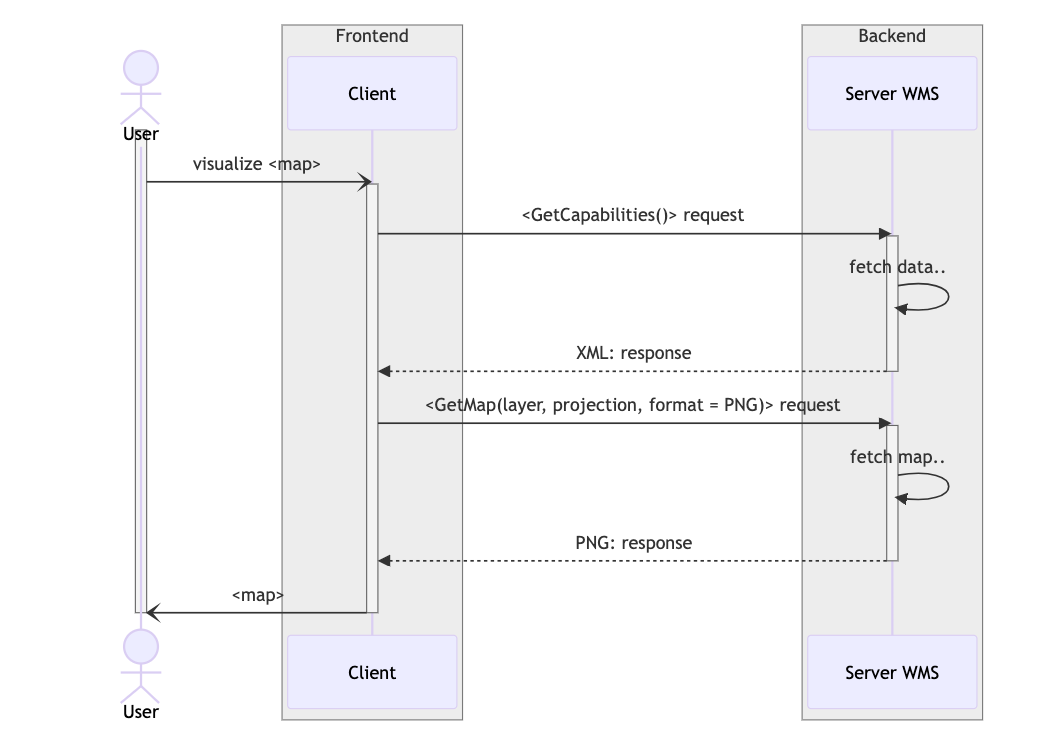
\includegraphics[width=1\textwidth]{images/Capitolo2/ProtocolWMS.png}
      \caption{Diagramma di Sequenza del protocollo WMS}
      \label{fig:wms protocol}
\end{figure}

\subsubsection{Formato della richiesta}

Lo standard specifica diversi tipi di richieste che possono essere effettuate ai server WMS:
\begin{itemize}
      \item \textit{GetCapabilities}: questa richiesta restituisce un documento XML che rappresenta le informazioni sul servizio WMS stesso, come il formato delle immagini delle mappe supportate, la compatibilità della versione del WMS e i layer disponibili, inclusi i dettagli come l'estensione geografica dei layer (bounding box), i sistemi di riferimento delle coordinate e l'opacità del layer.
      \item \textit{GetMap}: utilizzata per ottenere un'immagine di mappa dal servizio. I parametri inclusi nella richiesta comprendono l'estensione geografica della mappa, il sistema di coordinate, lo stile di rendering e il formato dell'immagine desiderato. La risposta alla richiesta è un'immagine rasterizzata della mappa desiderata, pronta per essere visualizzata su un browser web o in un'applicazione client.
\end{itemize}
I tipi di richiesta che i fornitori di WMS possono opzionalmente supportare includono:
\begin{itemize}
      \item \textit{GetFeatureInfo}: Consente di ottenere informazioni dettagliate su specifiche caratteristiche presenti sulla mappa. Restituisce informazioni associate a quella posizione, come punti di interesse o dati geografici particolari.
      \item  \textit{DescribeLayer}: Restituisce i tipi di feature disponibili per i layer specificati, che possono essere ulteriormente descritti utilizzando richieste Web Feature Service (WFS). Questa richiesta è utile per comprendere meglio la struttura e le caratteristiche dei dati geospaziali presenti nel servizio WMS.
      \item \textit{GetLegendGraphic}: Utilizzata per ottenere un'immagine della legenda della mappa, questa richiesta fornisce una guida visiva agli elementi presenti sulla mappa, come i simboli e le etichette dei layer.
\end{itemize}
Qui sotto è riportato uno \textit{snippet} che contiene alcuni esempi possibili di richieste WMS, eseguite utilizzando il comando CURL per simulare il comportamento di una richiesta HTTP.
% \texttt{WMS example requests}.
\lstinputlisting[language=bash]{listings/Capitolo2/wms-requests-example.sh}
Qui di seguito invece viene mostrato al lettore un esempio di richiesta funzionante, fatta durante il percorso di tirocinio, ai server WMS del Geoportale Nazionale, gestito dal Ministero dell'Ambiente e della Sicurezza Energetica.
Ciò serve per ottenere dati geospaziali relativi alla mappa che illustra l'area allagabile conforme al Piano di Gestione del Rischio di Alluvioni (PGRA) del 2021.
\lstinputlisting[language=bash]{listings/Capitolo2/wms-requests.sh}
Come si può vedere dal \href{http://wms.pcn.minambiente.it/ogc?map=/ms_ogc/WMS_v1.3/Vettoriali/Alluvioni_Estensione.map&service=wms&request=getCapabilities}{messaggio di risposta} in formato XML inviato dai loro Server,
Il servizio offre funzionalità standard come la richiesta di mappe (GetMap) e informazioni (GetFeatureInfo), oltre a supportare la descrizione dei layer (DescribeLayer) e la visualizzazione della legenda (GetLegendGraphic).
\\Per ulteriori informazioni dettagliate sullo standard WMS, è possibile fare riferimento alla documentazione ufficiale disponibile sul sito web di Open Geospatial Consortium \cite{DocumentazioneWMTS}

\subsection{Protocollo WMTS}

A differenza del WMS, il quale invia un'unica immagine per ogni mappa ai client, il WMTS la "segmenta" in piccole porzioni rettangolari, denominate \textit{tiles}.
\\Le tiles vengono prima pre-renderizzate e poi memorizzate sul server. Successivamente, sotto richiesta dei client, vengono recuperate e restituite come messaggio di risposta.
\\Quando un utente desidera visualizzare una mappa (nel nostro caso in un'applicazione web), il client invia tante richieste HTTP al server WMTS, una per ogni tile, specificando la porzione di mappa che vuole visualizzare, la proiezione e il formato dell'immagine desiderato. Il server, di conseguenza, risponde inviando le tiles corrispondenti alle richieste. Il client, appena ricevute le tiles, le combina insieme per formare la porzione di immagine effettiva di mappa richiesta.
\\Una delle principali caratteristiche del WMTS è che l'utilizzo delle tiles riduce la quantità di elaborazione richiesta dal server per mostrare correttamente la mappa.
Il server WMTS deve infatti fornire solo le tiles necessarie per l'area richiesta, anziché generare e inviare un'unica immagine completa. Così facendo, si riduce sia il carico di rete, sia la quantità di elaborazione di dati che il server deve eseguire, rendendolo più efficiente rispetto al server WMS.
\\Inoltre, le tiles aprono le porte ad una politica di caching: trattandosi di piccole porzioni di immagini, queste possono essere facilmente memorizzate nella cache. Sul lato back-end, infatti, il servizio WMTS può cachare le tiles più utilizzate e restituirle più rapidamente al client. Lato front-end, invece, il browser è in grado di intercettare le risposte inviate dal server e di memorizzare nella sua cache interna l'immagine della tile. In questo modo, quando il client richiede la stessa tile, quest'ultima viene visualizzata senza dover contattare nuovamente il server. Questo è possibile poichè le tiles sono di piccole dimensioni, e quindi il peso effettivo della richiesta è sufficiente da poter memorizzare la risposta nella cache del browser.
Questo consente di ridurre il carico di richieste sul server e di migliorare la velocità di caricamento delle mappe sui client.

\begin{figure}[htbp]
      \centering
      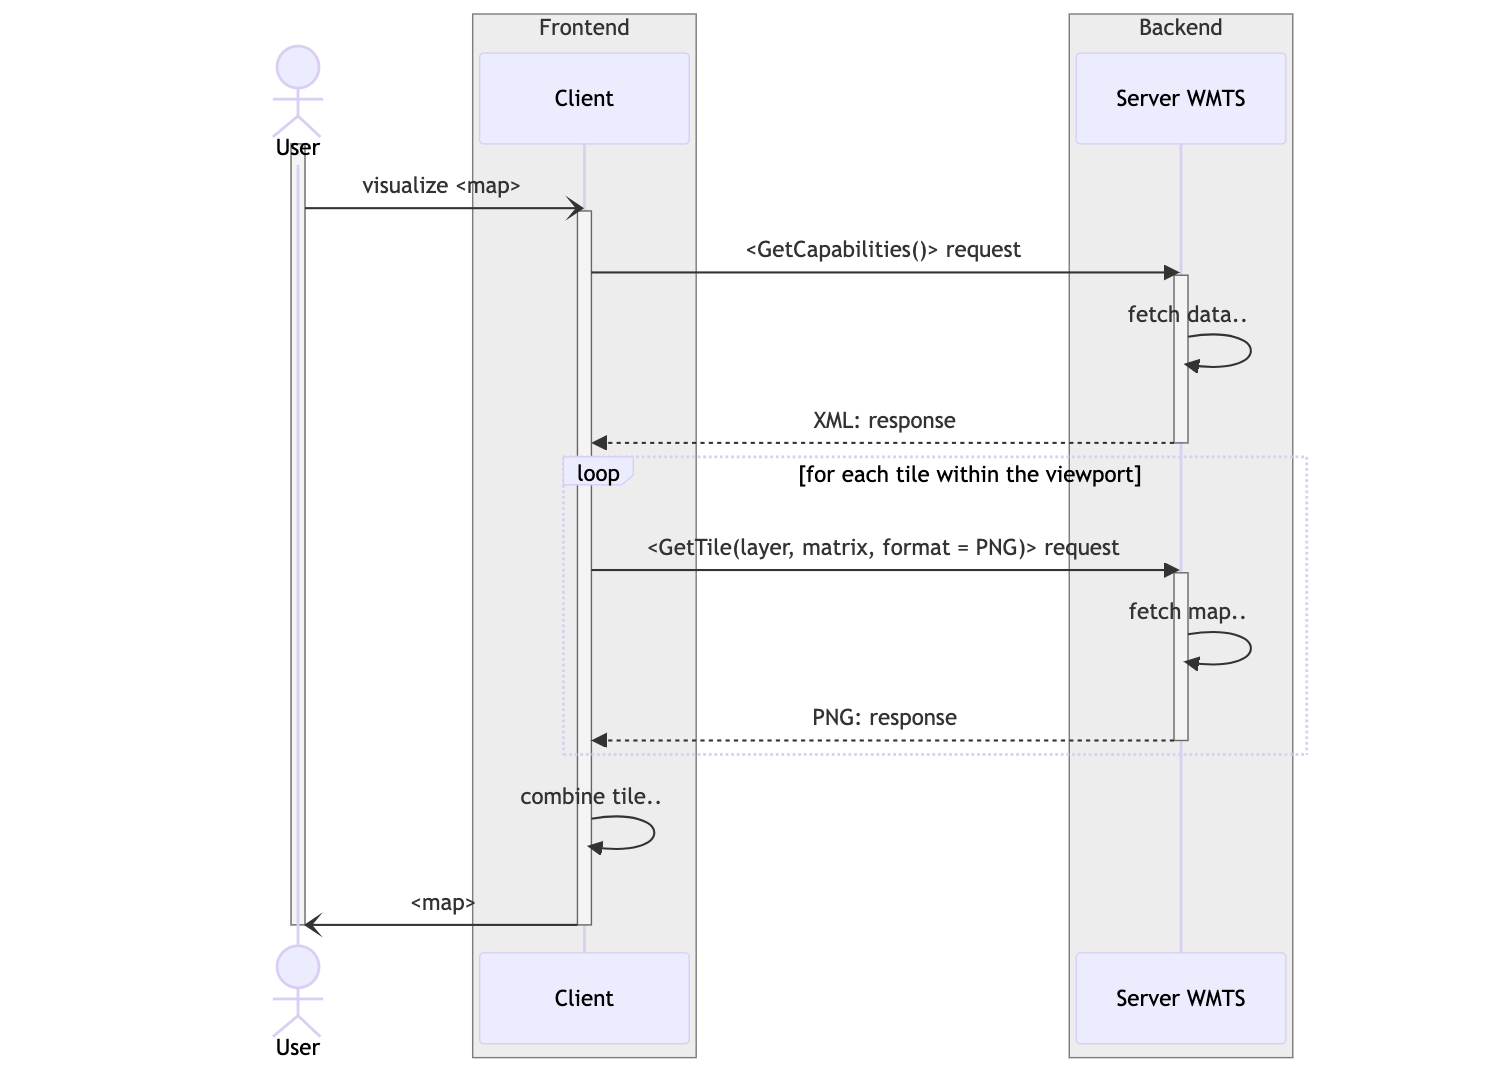
\includegraphics[width=1\textwidth]{images/Capitolo2/ProtocolWMTS.png}
      \caption{Diagramma di Sequenza del protocollo WMTS}
      \label{fig:wmts protocol}
\end{figure}

\subsubsection{Formato della richiesta}

\begin{itemize}
      \item \textit{GetCapabilities}: Restituisce un documento XML che descrive il \textit{Manifest} del servizio WMTS, inclusi i layers disponibili, i formati supportati, le coordinate di riferimento e altro ancora.
      \item \textit{GetTile}: Restituisce una Tile specifica in base alle coordinate geografiche e allo zoom specificato nella richiesta.
      \item \textit{GetFeatureInfo}: Questa richiesta non è molto comune nei servizi WMTS, in quanto genealmente viene direttamente utilizzata la richiesta GetFeatureInfo fornita dal servizio WMS. Se abilitata, questa richiesta restituisce informazioni aggiuntive associate a un tile, come attributi dei dati geospaziali presenti in quel punto della mappa.
\end{itemize}
Qui di seguito è riportato uno \textit{snippet} contenente alcuni esempi possibili di richieste WMTS, eseguite utilizzando il comando CURL per simulare il comportamento di una richiesta HTTP.

\lstinputlisting[language=bash]{listings/Capitolo2/wmts-requests-example.sh}
Per ulteriori informazioni dettagliate sullo standard WMTS, è possibile fare riferimento alla documentazione ufficiale disponibile sul sito web di Open Geospatial Consortium \cite{DocumentazioneWMTS}

\subsection{Protocollo WFS}

Il Web Feature Service (WFS) è un servizio web utilizzato per accedere e manipolare dati geospaziali attraverso internet.
A differenza di un WMS (Web Map Service), che fornisce mappe statiche sotto forma di immagini raster (come PNG o JPEG), un WFS offre dati geospaziali vettoriali, come punti, linee e poligoni che rappresentano oggetti geografici reali come edifici, strade e fiumi. Ogni singolo oggetto geografico è definito come una ``feature'' e può essere caratterizzato da una serie di attributi che ne descrivono le proprietà, come nome, altezza, larghezza e popolazione.
Similmente al WMS, che attraverso la richiesta GetMap può richiede una mappa specifica al server, il servizio WFS offre la richiesta GetFeature per richiedere una feature precisa che il server WFS provvederà a fornirgli.
\\I client possono anche eseguire operazioni di analisi spaziale, come il calcolo dell'area di un poligono o la ricerca delle feature più vicine a una determinata posizione.
Ad esempio, è possibile interrogare il servizio per ottenere informazioni su tutti gli edifici situati in una determinata area, oppure trovare tutti i fiumi di una certa lunghezza.
\\Queste informazioni vengono trasmesse utilizzando il formato GML (Geography Markup Language), che consente di descrivere in modo dettagliato la geometria e le proprietà di ciascuna feature.

\begin{figure}[htbp]
      \centering
      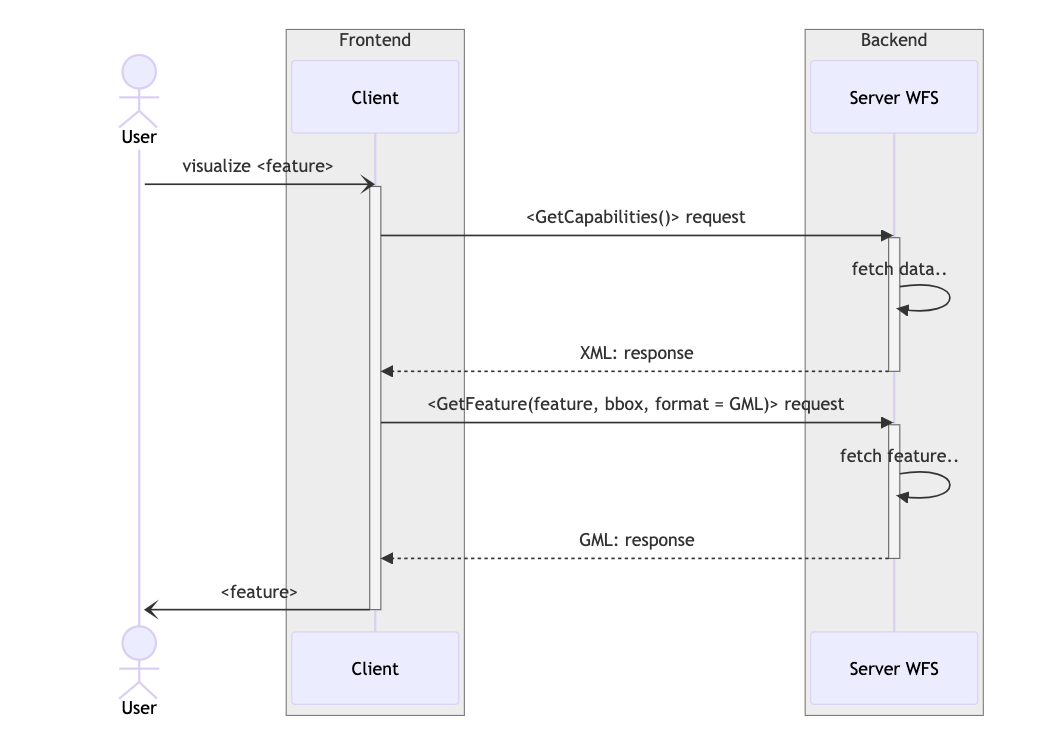
\includegraphics[width=1\textwidth]{images/Capitolo2/ProtocolWFS.png}
      \caption{Diagramma di Sequenza del protocollo WFS}
      \label{fig:wfs protocol}
\end{figure}

\subsubsection{Formato della richiesta}

Le richieste che è possibile fare a un servizio WFS (Web Feature Service) sono le seguenti:

\begin{itemize}
      \item \textit{GetCapabilities}: Come per i WMS, la richiesta GetCapabilities restituisce un documento XML che fornisce informazioni dettagliate sul servizio WFS stesso. Queste informazioni includono i tipi di feature supportati, i formati di trasmissione dei dati, i metodi di interrogazione supportati e altre capacità del servizio. Il documento XML include anche i dettagli sulle feature disponibili, gli attributi associati a ciascuna feature e le estensioni geografiche. Inoltre, fornisce informazioni sui sistemi di riferimento delle coordinate supportate e altre proprietà dei dati geografici disponibili.
      \item \textit{DescribeFeatureType}: è utilizzata per ottenere una descrizione dettagliata della struttura dei dati vettoriali (feature types) disponibili attraverso il servizio. In pratica, questa operazione fornisce informazioni sullo schema dei dati vettoriali, inclusi i tipi di attributi, i nomi dei campi e i tipi di geometria.
      \item \textit{GetFeature}: è una delle richieste principali nel protocollo WFS. Questa richiesta consente agli utenti di recuperare le feature geografiche in base a criteri specifici, come l'area di interesse, i tipi di feature o attributi desiderati. In pratica, tramite la richiesta GetFeature è possibile interrogare il servizio WFS per ottenere i dati geografici vettoriali corrispondenti a determinati parametri di ricerca. Ad esempio, è possibile richiedere tutte le strade in una determinata città, tutti gli edifici con una certa altezza o tutte le aree verdi in un parco.
\end{itemize}
I tipi di richiesta che i fornitori di WFS possono opzionalmente supportare si concentrano principalmente sulle feature, esse sono:
\begin{itemize}
      \item \textit{Transaction}: Consente agli utenti di modificare i dati geografici nel servizio WFS, consentendo operazioni di aggiornamento come l'aggiunta, la modificia o l'eliminazione di una feature. Ciò è particolarmente utile per gli utenti che necessitano di mantenere aggiornati i dati geografici all'interno del servizio, consentendo loro di interagire direttamente e apportare modifiche in tempo reale.
      \item \textit{LockFeature}: Consente agli utenti di acquisire un blocco di accesso esclusivo alle feature, impedendo ad altri utenti di modificarle durante determinate operazioni.
      \item \textit{GetPropertyValue}: Questa richiesta consente agli utenti di ottenere i valori degli attributi di una o più feature senza recuperare l'intera geometria delle feature stesse. È utile quando si desidera ottenere solo informazioni specifiche sugli attributi delle feature senza dover recuperare tutti i dettagli geometrici associati.
      \item \textit{GetFeatureWithLock}: viene usata per ottenere le feature con un blocco di accesso esclusivo in una singola operazione, combinando le funzionalità di GetFeature e LockFeature. Questo permette agli utenti di acquisire un blocco di accesso esclusivo alle feature desiderate prima di eseguire operazioni di interrogazione o aggiornamento su di esse.
\end{itemize}
Qui di seguito è riportato uno \textit{snippet} contenente alcuni esempi possibili di richieste WFS, eseguite utilizzando il comando CURL per simulare il comportamento di una richiesta HTTP.

% \texttt{WFS example requests}.
\lstset{basicstyle=\footnotesize\ttfamily}
\lstinputlisting[language=bash]{listings/Capitolo2/wfs-requests-example.sh}
Ecco un altro esempio di richiesta funzionante, effettuata sempre durante il percorso di tirocinio, ai server WFS del Geoportale Nazionale.
Come si può notare, questa richiesta è simile a quella effettuata precedentemente per il servizio WMS, ma questa volta viene rivolta al servizio WFS. Entrambi i servizi offrono informazioni sulla stessa mappa, ma con approcci diversi: mentre il WMS fornisce immagini della mappa, il WFS trasmette le feature geospaziali che compongono la mappa.

\lstset{basicstyle=\footnotesize\ttfamily}
\lstinputlisting[language=bash]{listings/Capitolo2/wfs-requests.sh}
Anche in questo caso, come si può vedere dal loro \href{http://wms.pcn.minambiente.it/ogc?map=/ms_ogc/wfs/Alluvioni_Estensione.map&service=wfs&request=getCapabilities}{messaggio di risposta} in formato XML inviato dai loro Server,
il servizio offre funzionalità standard come la richiesta di feature (GetFeature) e la descrizione dei tipi di feature (DescribeFeatureType), oltre a supportare la modifica dei dati geografici tramite transazioni (Transaction).
\\Per ulteriori informazioni dettagliate sullo standard WFS, è possibile fare riferimento alla documentazione ufficiale disponibile sul sito web di Open Geospatial Consortium \cite{DocumentazioneWMS}

\subsection{Protocollo WCS}

Infine, il Web Coverage Service (WCS) è uno standard creato per agevolare l'accesso e l'interrogazione di dati raster, comunemente denominati ``coperture'' o ``coverage''.
A differenza dei servizi convenzionali che forniscono solo immagini pre-renderizzate (come nel caso dei WMS), il WCS attraverso le coverage permette agli utenti di ottenere porzioni di immagini, divise in segmenti. Questi segmenti possono essere considerati come blocchi di dati geospaziali che rappresentano parti di una mappa o di un'immagine geografica più ampia. Le coverage semplificano quindi l'accesso ai dati, consentendo agli utenti di richiedere solo le porzioni di interesse senza dover scaricare l'intera immagine.
\\Inoltre, i servizi WCS possono anche comprendere informazioni aggiuntive come metadati e altre informazioni contestuali.

% Immagina di avere un dataset geospaziale che rappresenta la temperatura superficiale del mare in varie regioni oceaniche. Ogni pixel di questo dataset non rappresenta solo un valore numerico che indica la temperatura, ma è anche associato a informazioni semantiche che indicano, ad esempio, la data e l'ora dell'osservazione, la profondità a cui è stata effettuata l'osservazione, il tipo di strumento utilizzato per la misurazione e così via.
% Con un servizio come il WCS, è possibile accedere direttamente a questo dataset e richiedere informazioni specifiche. Ad esempio, potresti chiedere di restituire i valori di temperatura per una determinata area geografica in un intervallo di tempo specifico e a una profondità specifica. Il servizio restituirebbe quindi i dati grezzi, cioè i valori di temperatura insieme alle informazioni semantiche associate a ciascun punto dati.
% Ciò significa che non stai solo ottenendo un'immagine statica della temperatura, ma hai accesso ai dati sottostanti con tutte le informazioni aggiuntive che possono essere utilizzate per interpretare correttamente quei dati. Questo ti permette di eseguire analisi più avanzate, confrontare i dati con altre fonti, estrarre informazioni specifiche e altro ancora, in base alle tue esigenze.

% Il WCS fornisce i dati disponibili insieme alle loro descrizioni dettagliate; permette richieste complesse per questi dati e restituisce i dati con relativa semantica di origine (anziché le immagini) in modo da essere interpretato, estrapolato, ecc. e non solo disegnato. Questo servizio è l'alternativa al WFS, che restituisce i dati vettoriali, e al WMS che produce una immagine digitale.

\section{OSGeo, Tiled Map Service (TMS)}

Il protocollo Tiled Map Service (TMS), è un altro standard utilizzato per servire mappe geospaziali. A differenza di quelli sopra citati, questa specifica non è definita dall'Open Geospatial Consortium, ma è stata introdotta dall'Open Source Geospatial Foundation (OSGeo). Per questo motivo, nonostante entrambi i protocolli si occupano di fornire dati di mappe, presentano alcune differenze.
\\Questo standard può essere considerato come una semplificazione del servizio WMTS, in quanto continua a servire mappe geospaziali sotto forma di tiles, ma offre contemporaneamente meno funzionalità.
Infatti questo standard non richiede che il client debba prima ottenere informazioni sul servizio attraverso una richiesta simile a  \textit{GetCapabilities}. Il client può dedurre le informazioni sul servizio TMS dalla struttura dell'URL e può quindi accedere direttamente alle tiles della mappa tramite percorso URL, senza dover chiedere prima alcun tipo di informazioni al servizio stesso. Possiamo quindi affermare che la struttura degli URL di un servizio TMS segue una convenzione simile a quella delle cartelle: ogni livello di zoom della mappa e ogni tile è rappresentata da un URL univoco e questi possono essere organizzati in modo gerarchico, nello stesso modo delle cartelle in un File System.
\\Questo comporta da un lato un protocollo più semplice, ma dall'altro meno funzionalità: per esempio, il servizio non può fornirti informazioni su tutti i tipi di richieste a cui può essere interrogato. Nel caso di un servizio WMS, infatti, il client attraverso la GetCapabilities può capire o meno se il server supporta ulteriori richieste come GetFeatureInfo o GetLegendGraphic.
Inoltre, il protocollo TMS prevede solo la trasmissioni di immagini tile, non restituisce altri tipi di informazioni (come nel caso della GetFeatureInfo che restituisce informazioni aggiuntive insieme all'immagine di mappa).
\\Ciò può sembrare una cosa negativa, ma è importante tenere conto anche del peso delle richieste. Una richiesta di getCapabilities ad un servizio di mappe può restituire un messaggio di risposta molto grande e pesante, sopratutto se contiene molti layer (mappe) al suo interno. Durante il tirocinio è capitato per esempio di ricevere risposte di un peso oltre i 30MB. Anche se può sembrare insignificante, gestire un peso simile all'interno di servizi web risulta molto tedioso, specialmente dal punto di vista della memorizzazione nella cache del browser.
\\Inoltre, avere una struttura gerarchica simile a quella di un File System, può portare a tanti benifici. Uno di essi, ad esempio, è la facilità nel distribuire tutte le tiles all'interno di una CDN (Content Delivery Network), La stessa cosa può essere fatta anche nel caso dei servizi WMTS tramite query params, ma risulta molto più complesso e difficile da gestire. L'utilizzo di CDN può migliorare significativamente le prestazioni, l'affidabilità e la scalabilità del servizio, (?) possiamo utilizzare per esempio i bucket s3 di amazon. alleggeriscono il carico del server perché vengono spostati su altri server, l'utilizzo di bucket s3 tramite amazon permette con facilità la scalabilità del servizio, così da offrire la stessa mappa su più server. Affidabilià petché ci pensa amazon a rendere sicuri le mappe. Infine, le richieste di un servizio TMS sono più facili da memorizzare nella cache del browser rispetto al WMTS perché i suoi URL sono semplici e diretti. Al contrario, il WMTS spesso utilizza parametri più complessi nelle sue richieste, attraverso l'utilizzo dei query parameters, rendendo il memorizzazione nella cache del browser meno diretta e più soggetta a variazioni.
\\La struttura di una richiesta TMS per accedere ad una specifica tile è la seguente
\lstinputlisting[language=bash]{listings/Capitolo2/tms-requests-example.sh}
Questa richiesta restituisce direttamente una tile della mappa, generalmente grande 256x256, nel formato e proiezione richiesti. Le coordinate x e y rappresentano la posizione della tile all'interno della griglia, mentre la z il suo livello di zoom. Per ogni livello di zoom sono presenti dei confini, chiamati "bounding box" o "extent" che indicano l'estensione geografica delle tiles disponibili per quel livello di zoom. Se richieste delle tile al di fuori di questi confini, il server TMS restituisce un messaggio di errore.
\begin{figure}[htbp]
      \centering
      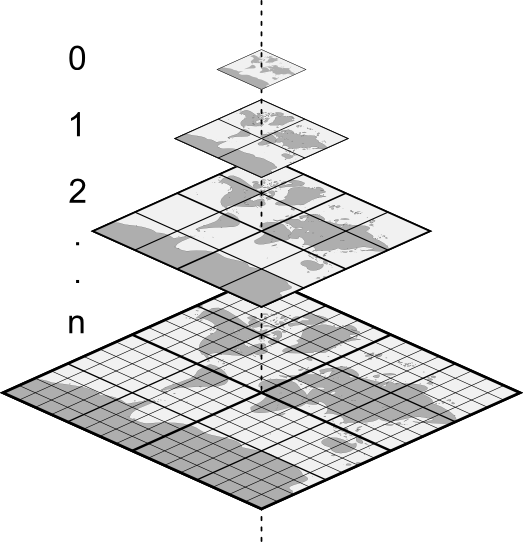
\includegraphics[width=0.5\textwidth]{images/Capitolo2/tilesPyramid.png}
      \caption{Tiles con livello di zoom}
      \label{fig:tmsTiles}
\end{figure}

\subsubsection{Formato della richiesta}

Come indicato nella specificata del servizio TMS \cite{DocumentazioneTMS}, esistono anche altre richieste che un client può effettuare per ottenere ulteriori informazioni oltre a quella relativa alle tiles. Le principali sono:
\begin{itemize}
      \item \textit{TileMapServiceResource}: questa richiesta è quella più simile a getCapabilities, permette di vedere tutte le mappe disponibili che il servizio TMS ha a disposizione, specificando il nome della mappa, il formato dell'immagine e la sua proiezione. Può anche essere fornita più volte la stessa mappa, con formati e proiezioni differenti. Un esempio di risposta a tale richiesta è la seguente:
            \lstset{basicstyle=\footnotesize\ttfamily}
            \lstinputlisting[language=xml]{listings/Capitolo2/TileMapServiceResource.xml}
      \item \textit{TileMapResource}: questa richiesta fornisce informazioni più dettagliate su una mappa, specificandone i confini, la dimensione delle tile, la proiezione e tutti i livelli di zoom disponibili che il client può richiedere (coordinata z) con i suoi rispettivi confini (extent). Un esempio di risposta a tale richiesta è la seguente:
            \lstset{basicstyle=\footnotesize\ttfamily}
            \lstinputlisting[language=xml]{listings/Capitolo2/TileMapResource.xml}
      \item \textit{TileResource}: la richiesta effettiva per richiedere la tile che corrispondete esattamente a quella spiegata in precedenza.
\end{itemize}
Il ciclo di vita di un client che richiede una mappa da un server TMS può essere descritto nel seguente modo:
Inizialmente, il client contatta tramite richiesta TileMapServiceResource un server TMS per ottenere le informazioni di tutte le mappe disponibili.
Dopo aver selezionato la mappa desiderata, il client utilizza la richiesta TileMapResource per ottenere tutti i possibili livelli di zoom, con i relativi confini.
A questo punto il client richiede direttamente le tiles della mappa desiderata attraverso le coordinate x, y e z, senza sforare dai confini. Il server risponde risponde con l'immagine della tile.

% spiegare che non è obbligatorio, per esempio nel tirocinio abbiamo fatto il map enumerator e abbiamo saltato il get tiles, perché essendo url le possiamo buttare da un altra parte? Ancora non è stato fatto quindi aspettiamo.

% nota per samuele futuro: ricordati di spiegare che le get capabilities pesano uno sfracello, e avere il map enumerator che ti restituisce tutto in json con i vari servizi di mappe, evita di fare questa richiesta

\section{Formati di file GeoSpaziali}
I formati di file geospaziali sono tipi di file utilizzati per memorizzare e scambiare dati geografici e spaziali. Questi dati possono includere informazioni come mappe, immagini satellitari, dati di altitudine, di utilizzo del suolo e molti altri. Alcuni dei formati di file geospaziali più comuni includono:
\begin{itemize}
      \item \textit {Shapefile} (.shp): è uno dei formati più diffusi per memorizzare dati geografici vettoriali, come punti, linee e poligoni. È stato sviluppato da ESRI e può essere utilizzato con una varietà di software GIS.
      \item \textit {GeoTIFF} (.tif): è una versione del formato di file TIFF (Tagged Image File Format) che include dati georeferenziati. È comunemente utilizzato per memorizzare immagini raster geograficamente riferite.
      \item \textit {GeoJSON} (.geojson): è un formato di file basato su JSON (JavaScript Object Notation) utilizzato per memorizzare dati geospaziali vettoriali. È spesso utilizzato per lo scambio di dati geografici su web e tra diversi software GIS.
      \item \textit {KML/KMZ} (.kml, .kmz): KML (Keyhole Markup Language) è un formato di file XML utilizzato per memorizzare dati geografici, come punti di interesse e percorsi. KMZ è una versione compressa di KML che include anche le risorse associate, come immagini e modelli 3D.
      \item \textit {GeoPackage} (.gpkg): è un formato di file standard OGC (Open Geospatial Consortium) per memorizzare dati geospaziali in un singolo file SQLite. Supporta dati vettoriali e raster e può includere anche metadati e stili. Rappresentano dei database geografici.
\end{itemize}
La diversità di formati esistenti non costituisce un problema per i client che necessitano di utilizzare dati geospaziali. Normalmente,
si tende a conservare dati sui server nei formati di cui sopra (principalmente, nel tirocinio, sono stati utilizzati Shapefile e GeoJson). Un server può supportare contemporaneamente più servizi (WMS, WMTS, WFS, TMS, etc..). Questo perché ciascuno di essi è in grado di convertire gli stessi dati di mappa iniziali in formati diversi, solitamente quelli richiesti dai client.
Ad esempio, WMS permette di richiedere una mappa in formato PNG, JPG e GIF. Quando viene effettuata una richiesta tramite questo servizio, questi accede ai dati conservati, ad esempio, in Shapefile, e li converte nel formato specificato. è da notare come non ci si debba necessariamente attenere ad uno dei servizi standard esistenti, ma si possa anche specificarne uno custom che permetta di restituire i dati iniziali in un formato scelto a proprio piacimento. Il caso più comune è che si vadano restituire i dati nel loro formato originario.

\section{OpenLayers}

OpenLayers è una libreria open source JavaScript che fornisce strumenti per la visualizzazione di mappe interattive su pagine web. Fornisce grande capacità di astrazione per gli sviluppatori, andando ad incapsulare tutte le funzionalità dei servizi menzionati fino ad ora.

\subsubsection{Caratteristiche Principali}
Una delle caratteristiche principali di OpenLayers è la sua capacità di offrire un interfaccia grafica di mappe omogenea su diversi tipi di dispositivi e browser. Essa permette, in modo intuitivo e coinciso, di accedere a una serie di funzionalità basilari, quali zoom, capacità di trascinare la mappa e interazione con elementi a schermo (come marker o punti).
\\Offre inoltre API ad alto livello che consentono di integrare facilmente diversi tipi di servizi geospaziali nei progetti, come WMS, WMTS, WFS, WCS, TMS etc..
Sono supportati anche formati strettamente geospaziali, tra cui GeoJSON, Shapefile, KML, GPX, etc.. L'accesso a questi dati è possibile sia contattando un server esterno, senza aver bisogno di utilizzare esplicitamente i servizi sopra citati, sia salvando i relativi file direttamente il locale per poi accedervi.
Tutti i sistemi di coordinate geografiche e proiezioni cartografiche sono disponibili in questa libreria, evitando di doverli calcolare da zero
\\Infine, OpenLayers supporta di default alcuni provider di mappe, tra cui: OpenStreetMap, Bing Maps, Google Maps, MapQuest etc.. Ciò non preclude la possibilità di utilizzare altri servizi di mappe esterni.
% \\OpenLayers offre allo sviluppatore la possibilità di personalizzare lo stile grafico dell'interfaccia grafica delle mappe, attraverso l'utilizzo di fogli di stile CSS e l'utilizzo di plugin

\subsubsection{Architettura di OpenLayer}

Essendo una libreria OpenSource, il codice di OpenLayers è interamente disponibile su Github \cite{GithubOpenLayers}.
\\Inoltre, come si può vedere dalla documentazione \cite{DocumentazioneOpenLayers}, l'architettura di OpenLayers è basata su un modello di programmazione modulare, in cui ogni modulo svolge precise funzionalità per la creazione e la gestione delle mappe. I moduli di OpenLayer principali sono:

\begin{itemize}
      \item ol/Map: è il core della libreria. Esso rappresenta la mappa stessa e fornisce funzionalità di base come la gestione dei layer, degli eventi e delle view.
      \item ol/View: questo modulo si occupa di gestire la View (la vista) della mappa, controlla la proiezione e il livello di zoom della mappa. La vista determina cosa viene mostrato sulla mappa e in quale modo.
      \item ol/layer: si occupa della creazione del layer sulla mappa, inclusi layer vettoriali, raster e di tile.
      \item ol/source: fornisce classi per definire le fonti di dati per i layer, ad esempio fonti WMS, WFS, GeoJSON, ecc.
      \item ol/control: viene utilizzato per la creazione di controlli e widget per la mappa, come strumenti per lo zoom, la scala, la misurazione delle distanze, ecc.
      \item ol/interaction: si occupa dell interazioni utente sulla mappa, come la selezione di una feature, lo zoom effettuato attraverso il dopppio click o lo scroll del mouse e altre azioni simili.
      \item ol/proj: Questo modulo gestisce la gestione dei sistemi di coordinate e delle proiezioni cartografiche.
\end{itemize}
OpenLayers supporta anche l'aggiunta di plugin di terze parti per estendere le sue funzionalità. Una raccolta di plugin è fornita sul loro sito al seguente \href{https://openlayers.org/3rd-party/}{link}.

\section{GeoServer}

GeoServer è un software OpenSource scritto in Java che permette di caricare e servire dati di mappe geospaziali.
All'interno di GeoServer i dati possono essere caricati in vari formati (come Shapefile, GeoPackage, etc..) per poi essere esposti attraverso l'utilizzo di protocolli standard OGC (come WMS, WFS, etc..), oppure attraverso l'utilizzo di altri protocolli come TMS.
Ad esempio, è possible caricare un file di mappa in formato Shapefile ed esporlo sul proprio server mediante un servizio WMS.
In questo modo un client che supporta tale protocollo (per esempio OpenLayer), può visualizzare la mappa interessata e richiederla in un formato raster come PNG, JPG o simili.

\subsubsection{Caratteristiche Principali}

Una funzionalità del GeoServer è il "mirroring" di servizi OGC, ovvero consente di replicare e mantenere aggiornati i servizi di mappe forniti da server esterni, i quali espongono i dati geospaziali tramite protocolli WMS, WFS, etc..
\\Ciò è possibile in quanto il GeoServer è in grado di memorizzare al suo interno l'URL che rappresenta la richiesta di \textit{GetCapabilities}. Come già spiegato, questa richiesta è essenziale per ottenere tutte le informazioni necessarie (layer di mappe, proiezioni, formati, etc..) al fine di richiedere le mappe fornite dal server esterno.
\\In pratica, ogni volta che un client richiede al GeoServer una mappa che non è presente localmente, il GeoServer inizia contattando il server esterno tramite una richiesta di GetCapabilities. Una volta ricevuta la risposta, il GeoServer esegue un'altra richiesta (ad esempio una GetMap nel caso dei servizi WMS) per ottenere la mappa specifica richiesta dal client. Una volta che il GeoServer riceve i dati della mappa dal server esterno, li invia al client come risposta alla sua richiesta originale.
% (no bibop) Così facendo, in pratica, ogni volta che un client chiede al GeoServer una mappa che in realtà non possiede, il GeoServer contatta prima il server esterno tramite GetCapabilities, poi una volta ricevuta la risposta, esegue un’ulteriore richiesta (per esempio una GetMap, nel caso dei WMS) per richiede la mappa che il client ha chiesto inizial mente al GeoServer. Una volta ottenuta la risposta, il GeoServer invia i dati della mappa sotto forma di risposta al client.
\\Questo consente di memorizzare tutti i dati delle mappe, potenzialmente anche esposte medianti protocolli diversi, sotto un unico server. Tale pratica non solo semplifica la gestione e la manutenzione dei dati geospaziali, ma dal punto di vista del client, viene offerta l'illusione che tutte le mappe siano contenute direttamente su un unico server.
\\Un'altra importante funzionalità di GeoServer è la capacità di esporre dati geospaziali utilizzando protocolli diversi. Ad esempio, è possibile registrare un servizio esterno di mappe WMS nel modo spiegato precedentemente per poi fornirlo come servizio WMTS o TMS, aumentandone così le prestazioni. In automatico il GeoServer si occuperà di fornire i della mappa in tiles, nonostante il servizio esterno non supporti questo formato. Questa caratteristica è particolarmente vantaggiosa per il fron-tend poiché elimina la necessità di supportare tutti i formati di dati.

\subsubsection{Meccanismi di Caching}

Avere tutte le mappe centralizzate sotto un unico server favorisce anche l'utilizzo di meccanismi di caching:
% Centralizzare le mappe su un unico servzio  semplifica notevolmente la gestione e il mantenimento dei dati geospaziali, in quanto non è più necessario cercare le mappe su diversi server esterni, riducendo così la complessità e il rischio di errori
a livello di WebServer, per esempio, tramite l'utilizzo di un Reverse Proxy, è possibile configurare politiche di caching per memorizzare temporaneamente le risposte alle richieste HTTP inviate dal GeoServer. Questo consente di ridurre il carico su di esso, in quanto alcune richieste possono essere soddisfatte direttamente dalla cache del WebServer senza doverle inoltrare nuovamente al GeoServer. Tale pratica risultarebbe più complessa da fare, se tutte le mappe fossero decentralizzate su servizi esterni, specialmente se di terze parti.
\\Inoltre, GeoServer stesso offre diversi livelli di caching, è possibile infatti configurarlo per memorizzare in una sua cache interna le risposte alle richieste di mappe.
\\Esiste anche la possibilità di memorizzare nella cache la risposta ottenuta dalla richiesta GetCapabilities inviata ai servizi OGC esterni, in modo da evitarne il recupero ogni volta. Questo risulta utile soprattutto quando si trattano mappe geospaziali che cambiano raramente nel tempo o che non cambiano affatto, anche se è possibile comunque rispolvere il problema in parte mettendo una cache di durata più breve.
Questo consente a GeoServer di rispondere più rapidamente alle richieste di mappe, utilizzando i dati già memorizzati nella cache anziché elaborarli nuovamente, riducendo così il carico e migliorando i tempi di risposta.
% nota per samuele del futuro: la cache è stata fatta perché altrimenti ci si beccava il rate limiting

\subsubsection{Architettura di GeoServer}

Geoserver supporta diversi tipi formati e servizi geospaziali, i più noti sono:

\begin{itemize}
      \item Servizi di mappe: WMS, WMTS, WFS, WCS, TMS per i servizi di mappe;
      \item Dati raster: GeoPackage, ArcGrid, GeoTIFF, ImageMosaic, WorldImage;
      \item Dati vettoriali o a oggetti geospaziali: ShapeFiles, GeoPackage, PostGIS;
\end{itemize}
% GeoServer is a web application, supporting any common servlet container (a standalone distribution is available with the Jetty (web server) as an embedded server). GeoWebCache, a Java-based caching component similar to TileCache, is bundled with GeoServer, but available separately.[7] Similarly, GeoServer packages GeoTools as a Java library, but it is also available separately.[8]
Questi ultimi possono essere caricati e gestiti tramite l'utilizzo di un'interfaccia grafica, realizzata sotto forma di un'applicazione web, oppure tramite l'utilizzo di chiamate ad una REST API.
\\Al fine di poter caricare correttamente una mappa all'interno di GeoServer, è necessario creare tre componenti basilari:
\begin{itemize}
      \item Workspace: rappresenta precisamente l'"area di lavoro", cioè il luogo in cui tutte le mappe vengono effettivamente caricate, quest'utlime a sua volta vengono organizzate in all'interno di Storage. Una workspace può contenere uno o più Storage.
      \item Storage: rappresenta il tipo di servizio di mappa che si vuole caricare all'interno di GeoServer. Può essere un servizio WMS, WFS, WCS, o un tipo di dato geospaziale come Shapefile, GeoTIFF, etc.. Ovviamente in base al tipo di Storage che si va a creare, le impostazioni visualizzate sull'interfaccia grafica (o i query param da inviare secondo la rest API) saranno differenti. Per esempio, se si va a creare un servizio esterno WMS, sarà chiesto il link delle capabilities da contattare. Se si andrà a caricare uno Shapefile, sarà richiesto il percorso locale in cui il file si trova.
      \item Layer: rappresenta la mappa effettiva, quella che verrà poi fornita al Front-end. È ciò che restituisce lo storage una volta ricevuta la risposta alla getCapabilities, nel caso di un servizio OGC, o ciò che contiene uno Shapefile. Ovviamente più layer possono stare all'interno di uno storage.
\end{itemize}
Dal punto di vista di architetturale, come si può vedere su Github \cite{GithubGeoServer}, GeoServer è stato sviluppato utilizzando Spring come Framework Java, e viene utilizzato per gestire tutte le funzionalità sopra citate. Anche la REST API è stata implementata sempre tramite Spring (Spring MVC Framework), mentre l'interfaccia grafica è stata realizzata invece tramite l'utilizzo di Wicket.
% Warning The API is documented as Swagger 2.0 files. However, these files have been written by hand back in 2017, and have not always been kept up to date with the evolution of the GeoServer configuration object structure. Also, they have not been tested for proper client generation, and will likely not work for that purpose. Take them only as a form of documentation.
% \\Tuttavia, come si può leggere dalla documentazione, la REST API non solo non è ancora stata aggiornata allo standard di OpenAPI 3 (rimanendo ancora ferma Swagger 2.0), ma non rispetta nemmeno
\\Tutta via, come viene riportato dagli sviluppatori di GeoServer nella loro documentazione \cite{DocumentazioneGeoServer}, la REST API presenta alcune criticità importanti che possono influenzare il suo utilizzo e la sua affidabilità.
Innanzitutto, la specifica della REST API è rimasta alla versione di Swagger 2.0 e non è aggiornata allo al nuovo standard di OpenAPI 3.0, ciò comporta ad una peggiore comprensione e utilizzo dell'API stessa.
Ma soprattuto, viene fatto notare che i file di Swagger utilizzati per documentare l'API sono stati creati manualmente nel 2017 e non sono stati più aggiornati con l'evoluzione dell'infrastruttura del software.
\\L'utilizzo dell'API di GeoServer è stata una parte cruciale durante periodo di tirocinio, e questo problema ha rappresentato una sfida significativa, in quanto è stato necessario sistemare manualmente le richieste al fine di poterle utilizzare correttamente utilizzare correttamente.
% Questo processo è stato non solo laborioso e impegnativo, ma ha anche richiesto una profonda comprensione della struttura dell'API e dei suoi requisiti. Tuttavia, nonostante le difficoltà incontrate, ho potuto apprezzare appieno il valore dell'API di GeoServer e il suo ruolo fondamentale nel contesto del mio lavoro di tirocinio.